%======================================================================
\section{Certificado de optimalidad global en lazo cerrado (F7)}\label{sec:f7}
%======================================================================
\paragraph{Qué falta en la auditoría.} La auditoría de la sección~\ref{sec:auditoria} compara
cada decisión con el \emph{mejor plan encontrado} entre seis soluciones locales. Eso es una cota
superior (UB) del óptimo global $J^\star$, y no descarta que exista un plan mejor que ningún
arranque encontró. La certificación del P0 en lazo abierto (sección~\ref{sec:certificacion})
resolvió el problema con una cota inferior (LB) rigurosa, pero sólo en dos consultas y con
brechas de 2.3 y 11.4\,\%. Esta sección lleva esa cota a un subconjunto de consultas de lazo
cerrado y la ajusta con un \emph{branch and bound} espacial hasta una brecha de 0.01\,\%.

\paragraph{Qué certifica una cota inferior.} Si $LB\le J^\star\le UB$, entonces para la
decisión $u$ de cualquier formulación se cumple
\[
J(u)-J^\star\;\le\;J(u)-LB ,
\]
de modo que una sola LB certifica a la vez cuánto puede distar del óptimo global cada una de
N1, N2 y N3. Un solver local (Ipopt, Knitro) o un multistart sólo pueden bajar la UB: aportan
evidencia, pero no una prueba. La LB necesita una relajación.

\paragraph{La cota trivial.} El costo es una suma de cuadrados, así que $LB=0$ vale siempre. En
las consultas en que el mejor plan tiene $J\approx0$ (la planta ya está en la consigna: el
55--80\,\% de las consultas auditadas por F6), esa cota certifica una brecha absoluta igual a
$J$. Por eso la auditoría reportó distancias en kelvin y no brechas relativas. Las consultas
interesantes son las demás.

\subsection{Método}
\begin{enumerate}
  \item \textbf{El problema certificado} es exactamente el que resuelve N3 en el lazo: costo P0,
        ROM implícito convergido, caja del actuador y rampa dura $|u_k-u_{k-1}|\le5$~kg/s desde el
        caudal aplicado (\code{julia/F7Cert.jl}).
  \item \textbf{Reducción de la caja por la rampa.} Con la rampa dura, $u_k$ no puede salir de
        $[\dot m_{\rm prev}-5k,\ \dot m_{\rm prev}+5k]$. La propagación hacia adelante y hacia atrás
        achica la caja de 0--5543~kg/s del actuador físico a un ancho medio de 35--135~kg/s.
  \item \textbf{Cotas superiores.} Se evalúan las decisiones del lazo (N3), de N1 y de N2, y un
        multistart de Ipopt desde 24 arranques (las tres decisiones, uno en frío y 20 caminatas
        aleatorias factibles). Ipopt devuelve puntos que violan la rampa en unos $4\cdot10^{-7}$
        (su tolerancia); como sólo un punto exactamente factible es una UB válida, cada punto se
        proyecta antes de evaluarlo, lo que cambia $J$ en menos de $10^{-6}$.
  \item \textbf{Cota inferior por B\&B espacial.} En cada nodo (una sub-caja) se encierra el
        residuo del modelo afín con aritmética de intervalos (proposición~\ref{prop:taylor}) y se
        resuelve la relajación convexa de la proposición~\ref{prop:lb}, ahora con la rampa dura
        como restricción lineal. Se elige el nodo de menor LB, se parte por la variable de mayor
        $(\mathrm{ancho})\times(K-j+1)$, porque los pasos tempranos acumulan residuo en todo el
        horizonte, y se poda todo nodo con $LB\ge UB$. El punto de cada relajación se evalúa como
        candidato a UB. Si el encierro de un nodo no se verifica, el nodo hereda la LB del padre
        y se sigue partiendo. La LB global, el mínimo sobre los nodos abiertos, es válida en
        cualquier momento, aunque se agote el tiempo.
  \item \textbf{Subconjunto.} Diez semillas por familia (nominal a 40~kg/s, fallas del DET a
        40~kg/s, extrema con actuador físico) y, en cada una, hasta tres consultas auditadas
        por F6 con $J>0.01$ (la primera, una intermedia y la última). Para reproducir
        exactamente las consultas, se re-corre el lazo N3 de F6 con un gancho que las captura
        (\code{CAPTURE} en \code{julia/F6Tasks.jl}) y se guardan serializadas en
        \code{results/f7\_cert/queries/}. El B\&B tiene 900~s por consulta, en Olab.
\end{enumerate}

\subsection{Resultados}

\begin{table}[H]\centering\footnotesize\setlength{\tabcolsep}{3.5pt}
\begin{tabularx}{\linewidth}{@{}l r r r r r r r@{}}\toprule
Familia & Consultas & \multicolumn{2}{c}{Certificadas a} & \multicolumn{2}{c}{Brecha final} & Brecha & Exceso N1\\
\cmidrule(lr){3-4}\cmidrule(lr){5-6}
& & 0.01\,\% & 0.5\,\% & mediana & máx. & raíz (med.) & máx.\\\midrule
Nominal, 40~kg/s & 20 & 5 & 20 & 0.058\,\% & 0.50\,\% & 4.9\,\% & 0.51\,\%\\
Fallas del DET, 40~kg/s & 27 & 15 & 27 & 0.010\,\% & 0.12\,\% & 7.5\,\% & 0.15\,\%\\
Extrema, actuador físico & 30 & 22 & 30 & 0.010\,\% & 0.13\,\% & 100\,\% & 1.27\,\%\\\bottomrule
\end{tabularx}
\caption{Certificado de optimalidad global en 77 consultas de lazo cerrado (\code{results/f7\_cert/summary.md}).
Brecha: $(UB-LB)/UB$. «Raíz»: brecha antes de ramificar; en la familia extrema el encierro de la
caja completa no se verifica (raíz con $LB=0$) y la cota aparece al partir. Exceso N1: cota
certificada de $(J(u_{\rm N1})-J^\star)/UB$. La UB coincide con el costo de la decisión N3 del
lazo a menos de $10^{-9}$ relativo en todas las consultas.}
\label{tab:f7}
\end{table}

\begin{figure}[H]\centering
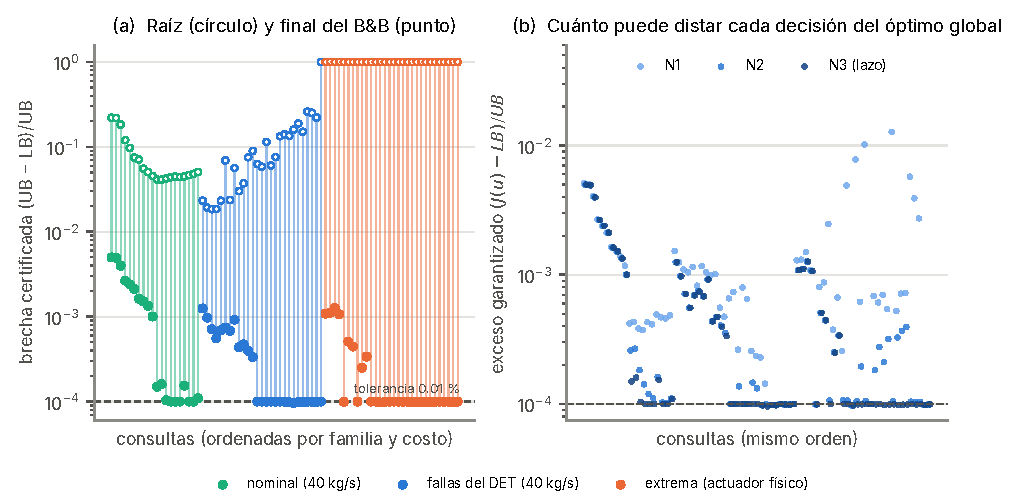
\includegraphics[width=\linewidth]{figures/fig_f7_certificate.pdf}
\caption{(a) Brecha certificada en la raíz (círculo) y al final del B\&B (punto), por consulta. La
línea de trazos es la tolerancia de 0.01\,\%; los puntos sobre ella son consultas certificadas
antes de los 900~s. (b) Exceso garantizado sobre el óptimo global de las decisiones N1, N2 y N3:
$(J(u)-LB)/UB$, es decir, la brecha más la diferencia de costo frente a la mejor decisión.}
\label{fig:f7-cert}
\end{figure}

\begin{figure}[H]\centering
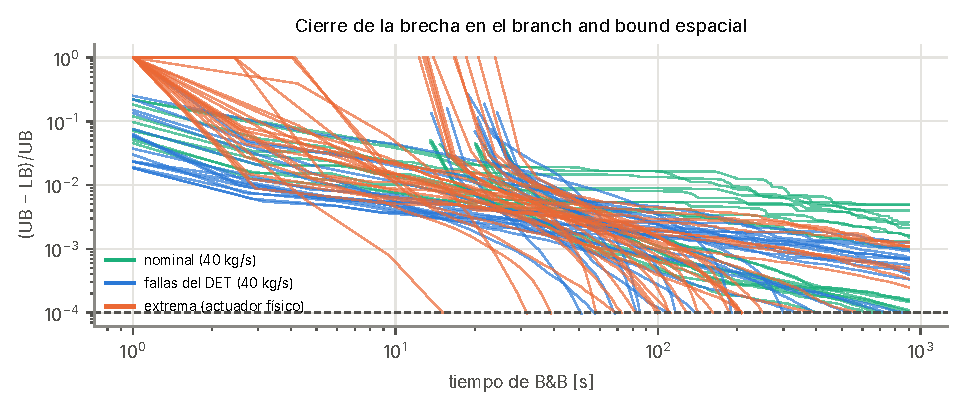
\includegraphics[width=\linewidth]{figures/fig_f7_convergence.pdf}
\caption{Cierre de la brecha durante el B\&B, una curva por consulta. Las curvas que empiezan en
1 son las de raíz no verificada (familia extrema); la brecha baja en unas pocas decenas de
segundos en cuanto las cajas se achican.}
\label{fig:f7-conv}
\end{figure}

\paragraph{Lectura.}
\begin{enumerate}
  \item \textbf{La decisión de N3 en el lazo es el óptimo global} en las 77 consultas, dentro de
        la brecha certificada: a menos de 0.01\,\% en 42 consultas y a menos de 0.5\,\% en
        todas. Las 35 consultas que no llegan a 0.01\,\% en 900~s tienen costos pequeños
        ($J\le32$) y una brecha absoluta de $\le0.01$, equivalente a un error RMS de la PCT de
        $\le0.02$~K en el horizonte. El caso más flojo, la consulta 11 de la familia nominal
        (0.5\,\% de un $J=0.025$), equivale a 0.002~K.
  \item \textbf{No hay otros óptimos locales.} Los 24 arranques de Ipopt convergen al mismo plan
        en todas las consultas (diferencias relativas de $10^{-8}$, del orden de la proyección
        de factibilidad), y ninguno mejora la decisión del lazo en más de $9\cdot10^{-10}$
        relativo. El B\&B confirma con una cota lo que el multistart sugiere.
  \item \textbf{N2 está certificado igual que N3} (su costo excede al de N3 en a lo más
        $1\cdot10^{-4}$ relativo), y \textbf{N1, a menos de 1.3\,\%} del óptimo global; su peor
        caso está en la familia extrema, donde la linealización alrededor de un punto fijo es
        menos exacta (sección~\ref{sec:trayectorias}). La mediana del exceso de N1 es de 0.07--0.08\,\%.
  \item \textbf{La relajación de la raíz es floja, pero la ramificación la ajusta rápido.} En la
        raíz la brecha es del 5--8\,\% (y no se verifica en la familia extrema, cuya caja es la
        más ancha). Con unos 4300 nodos (mediana) baja a la tolerancia: el residuo del modelo afín
        cae con el cuadrado del ancho de la caja, como ya mostraban las sub-cajas de la sección~\ref{sec:certificacion}.
\end{enumerate}

\paragraph{Knitro.} El plan incluye resolver las mismas consultas con Knitro (cuatro algoritmos y su
multistart), como confirmación independiente de la UB con otro solver
(\code{julia/f7\_knitro.jl}, sobre las consultas serializadas). Knitro~16 se instala en ambos
equipos, pero falta la licencia. Su resultado sólo puede bajar la UB, y un valor bajo la LB
certificada revelaría un error en alguna de las dos cotas.

\takeaway{\textbf{Respuesta a Q7 (segunda parte): certificado de optimalidad global en lazo cerrado.} En 77 consultas difíciles
de las tres familias, un \emph{branch and bound} espacial con encierros rigurosos por intervalos
demuestra que la decisión de N3 está a menos del 0.5\,\% del óptimo global (a menos del 0.01\,\%
en 42), que N2 tiene la misma garantía y que N1 está a menos del 1.3\,\%. Junto con la cota
trivial $J\ge0$, que certifica las consultas con $J\approx0$, esto cubre el resto de la auditoría.
Para el paper, «óptimo local» pasa a ser «óptimo global con brecha certificada».}

